\PassOptionsToPackage{unicode=true}{hyperref} % options for packages loaded elsewhere
\PassOptionsToPackage{hyphens}{url}
\PassOptionsToPackage{dvipsnames,svgnames*,x11names*}{xcolor}
%
\documentclass[ignorenonframetext,]{beamer}
\usepackage{pgfpages}
\setbeamertemplate{caption}[numbered]
\setbeamertemplate{caption label separator}{: }
\setbeamercolor{caption name}{fg=normal text.fg}
\beamertemplatenavigationsymbolsempty
% Prevent slide breaks in the middle of a paragraph:
\widowpenalties 1 10000
\raggedbottom
\setbeamertemplate{part page}{
\centering
\begin{beamercolorbox}[sep=16pt,center]{part title}
  \usebeamerfont{part title}\insertpart\par
\end{beamercolorbox}
}
\setbeamertemplate{section page}{
\centering
\begin{beamercolorbox}[sep=12pt,center]{part title}
  \usebeamerfont{section title}\insertsection\par
\end{beamercolorbox}
}
\setbeamertemplate{subsection page}{
\centering
\begin{beamercolorbox}[sep=8pt,center]{part title}
  \usebeamerfont{subsection title}\insertsubsection\par
\end{beamercolorbox}
}
\AtBeginPart{
  \frame{\partpage}
}
\AtBeginSection{
  \ifbibliography
  \else
    \frame{\sectionpage}
  \fi
}
\AtBeginSubsection{
  \frame{\subsectionpage}
}
\usepackage{lmodern}
\usepackage{amssymb,amsmath}
\usepackage{ifxetex,ifluatex}
\usepackage{fixltx2e} % provides \textsubscript
\ifnum 0\ifxetex 1\fi\ifluatex 1\fi=0 % if pdftex
  \usepackage[T1]{fontenc}
  \usepackage[utf8]{inputenc}
  \usepackage{textcomp} % provides euro and other symbols
\else % if luatex or xelatex
  \usepackage{unicode-math}
  \defaultfontfeatures{Ligatures=TeX,Scale=MatchLowercase}
\fi
% use upquote if available, for straight quotes in verbatim environments
\IfFileExists{upquote.sty}{\usepackage{upquote}}{}
% use microtype if available
\IfFileExists{microtype.sty}{%
\usepackage[]{microtype}
\UseMicrotypeSet[protrusion]{basicmath} % disable protrusion for tt fonts
}{}
\IfFileExists{parskip.sty}{%
\usepackage{parskip}
}{% else
\setlength{\parindent}{0pt}
\setlength{\parskip}{6pt plus 2pt minus 1pt}
}
\usepackage{xcolor}
\usepackage{hyperref}
\hypersetup{
            pdftitle={Lecture 1 - issues raised by missing data, a systematic approach, and missingness mechanisms},
            pdfauthor={Jonathan Bartlett (thestatsgeek.com)},
            colorlinks=true,
            linkcolor=blue,
            filecolor=Maroon,
            citecolor=Blue,
            urlcolor=blue,
            breaklinks=true}
\urlstyle{same}  % don't use monospace font for urls
\newif\ifbibliography
\usepackage{color}
\usepackage{fancyvrb}
\newcommand{\VerbBar}{|}
\newcommand{\VERB}{\Verb[commandchars=\\\{\}]}
\DefineVerbatimEnvironment{Highlighting}{Verbatim}{commandchars=\\\{\}}
% Add ',fontsize=\small' for more characters per line
\usepackage{framed}
\definecolor{shadecolor}{RGB}{248,248,248}
\newenvironment{Shaded}{\begin{snugshade}}{\end{snugshade}}
\newcommand{\AlertTok}[1]{\textcolor[rgb]{0.94,0.16,0.16}{#1}}
\newcommand{\AnnotationTok}[1]{\textcolor[rgb]{0.56,0.35,0.01}{\textbf{\textit{#1}}}}
\newcommand{\AttributeTok}[1]{\textcolor[rgb]{0.77,0.63,0.00}{#1}}
\newcommand{\BaseNTok}[1]{\textcolor[rgb]{0.00,0.00,0.81}{#1}}
\newcommand{\BuiltInTok}[1]{#1}
\newcommand{\CharTok}[1]{\textcolor[rgb]{0.31,0.60,0.02}{#1}}
\newcommand{\CommentTok}[1]{\textcolor[rgb]{0.56,0.35,0.01}{\textit{#1}}}
\newcommand{\CommentVarTok}[1]{\textcolor[rgb]{0.56,0.35,0.01}{\textbf{\textit{#1}}}}
\newcommand{\ConstantTok}[1]{\textcolor[rgb]{0.00,0.00,0.00}{#1}}
\newcommand{\ControlFlowTok}[1]{\textcolor[rgb]{0.13,0.29,0.53}{\textbf{#1}}}
\newcommand{\DataTypeTok}[1]{\textcolor[rgb]{0.13,0.29,0.53}{#1}}
\newcommand{\DecValTok}[1]{\textcolor[rgb]{0.00,0.00,0.81}{#1}}
\newcommand{\DocumentationTok}[1]{\textcolor[rgb]{0.56,0.35,0.01}{\textbf{\textit{#1}}}}
\newcommand{\ErrorTok}[1]{\textcolor[rgb]{0.64,0.00,0.00}{\textbf{#1}}}
\newcommand{\ExtensionTok}[1]{#1}
\newcommand{\FloatTok}[1]{\textcolor[rgb]{0.00,0.00,0.81}{#1}}
\newcommand{\FunctionTok}[1]{\textcolor[rgb]{0.00,0.00,0.00}{#1}}
\newcommand{\ImportTok}[1]{#1}
\newcommand{\InformationTok}[1]{\textcolor[rgb]{0.56,0.35,0.01}{\textbf{\textit{#1}}}}
\newcommand{\KeywordTok}[1]{\textcolor[rgb]{0.13,0.29,0.53}{\textbf{#1}}}
\newcommand{\NormalTok}[1]{#1}
\newcommand{\OperatorTok}[1]{\textcolor[rgb]{0.81,0.36,0.00}{\textbf{#1}}}
\newcommand{\OtherTok}[1]{\textcolor[rgb]{0.56,0.35,0.01}{#1}}
\newcommand{\PreprocessorTok}[1]{\textcolor[rgb]{0.56,0.35,0.01}{\textit{#1}}}
\newcommand{\RegionMarkerTok}[1]{#1}
\newcommand{\SpecialCharTok}[1]{\textcolor[rgb]{0.00,0.00,0.00}{#1}}
\newcommand{\SpecialStringTok}[1]{\textcolor[rgb]{0.31,0.60,0.02}{#1}}
\newcommand{\StringTok}[1]{\textcolor[rgb]{0.31,0.60,0.02}{#1}}
\newcommand{\VariableTok}[1]{\textcolor[rgb]{0.00,0.00,0.00}{#1}}
\newcommand{\VerbatimStringTok}[1]{\textcolor[rgb]{0.31,0.60,0.02}{#1}}
\newcommand{\WarningTok}[1]{\textcolor[rgb]{0.56,0.35,0.01}{\textbf{\textit{#1}}}}
\usepackage{longtable,booktabs}
\usepackage{caption}
% These lines are needed to make table captions work with longtable:
\makeatletter
\def\fnum@table{\tablename~\thetable}
\makeatother
\usepackage{graphicx,grffile}
\makeatletter
\def\maxwidth{\ifdim\Gin@nat@width>\linewidth\linewidth\else\Gin@nat@width\fi}
\def\maxheight{\ifdim\Gin@nat@height>\textheight\textheight\else\Gin@nat@height\fi}
\makeatother
% Scale images if necessary, so that they will not overflow the page
% margins by default, and it is still possible to overwrite the defaults
% using explicit options in \includegraphics[width, height, ...]{}
\setkeys{Gin}{width=\maxwidth,height=\maxheight,keepaspectratio}
\setlength{\emergencystretch}{3em}  % prevent overfull lines
\providecommand{\tightlist}{%
  \setlength{\itemsep}{0pt}\setlength{\parskip}{0pt}}
\setcounter{secnumdepth}{0}

% set default figure placement to htbp
\makeatletter
\def\fps@figure{htbp}
\makeatother


\title{Lecture 1 - issues raised by missing data, a systematic approach, and
missingness mechanisms}
\providecommand{\subtitle}[1]{}
\subtitle{Multiple imputation techniques for working with missing data}
\author{\href{https://thestatsgeek.com}{Jonathan Bartlett (thestatsgeek.com)}}
\date{Copenhagen, March 2020}

\begin{document}
\frame{\titlepage}

\begin{frame}
\tableofcontents[hideallsubsections]
\end{frame}
\begin{frame}{Course aims}
\protect\hypertarget{course-aims}{}

\begin{itemize}
\tightlist
\item
  Understand the effects of missing data on statistical analyses
\item
  Learn about the assumptions under which simple methods for handling
  missing data are valid
\item
  Learn about principled statistical methods for handling missing data,
  specifically multiple imputation
\end{itemize}

\end{frame}

\hypertarget{missing-data---whats-the-big-deal-and-a-systematic-approach}{%
\section{Missing data - what's the big deal and a systematic
approach}\label{missing-data---whats-the-big-deal-and-a-systematic-approach}}

\begin{frame}{Why is this necessary?}
\protect\hypertarget{why-is-this-necessary}{}

\begin{itemize}
\tightlist
\item
  Missing data commonly arise in empirical research.
\item
  They cause a loss of information, and arguably more importantly, may
  introduce bias into inferences.
\item
  They are often inadequately handled in both observational and
  experimental studies.
\item
  For example, (Karahalios et al.
  \protect\hyperlink{ref-karahalios2012review}{2012}) reviewed the
  reporting and handling of missing data in longitudinal measurements in
  cohort studies.
\item
  They found that reporting of missing data was inconsistent and
  inappropriate statistical methods continue to be used (in this field
  at least).
\item
  Scientific journals and bodies increasingly recognise the importance
  of careful handling of missing data.
\end{itemize}

\end{frame}

\begin{frame}{Missing data in trials - the problem and its prevention}
\protect\hypertarget{missing-data-in-trials---the-problem-and-its-prevention}{}

\begin{itemize}
\tightlist
\item
  A US National Research Council (NRC) report was recently published on
  the prevention and treatment of missing data in trials (Council
  \protect\hyperlink{ref-NRC2010}{2010}; Little et al.
  \protect\hyperlink{ref-Little2012}{2012}).
\item
  They noted that missing data have seriously compromised inferences
  from clinical trials in the past.
\item
  They concluded that the assumption that analysis methods can
  compensate for missing data are not justified.
\item
  The panel therefore recommended strategies for minimizing missing data
  in trials.
\end{itemize}

\end{frame}

\begin{frame}{Missing data in trials - six recommended principles
(steps)}
\protect\hypertarget{missing-data-in-trials---six-recommended-principles-steps}{}

Based on (Little et al. \protect\hyperlink{ref-Little2012}{2012})

\begin{enumerate}
\tightlist
\item
  Find out if values are missing are relevant for the intended analysis.
\item
  Formulate a well defined causal primary measure of treatment effect.
\item
  Document and investigate the reasons for missing data.
\item
  Decide on a primary set of assumptions about missing data.
\item
  Perform an analysis using a statistical method which is valid under
  the assumption chosen in 4.
\item
  Perform a sensitivity analysis to explore robustness to plausible
  deviations from the assumption in 4.
\end{enumerate}

\end{frame}

\begin{frame}{A principled approach}
\protect\hypertarget{a-principled-approach}{}

\begin{itemize}
\tightlist
\item
  We will attempt to follow such an approach.
\item
  Thinking more generally, outside of clinical trials, step 2. consists
  of specifying our substantive model or quantitiy of interest.
\end{itemize}

\end{frame}

\begin{frame}{Example}
\protect\hypertarget{example}{}

\begin{itemize}
\tightlist
\item
  e.g.~consider the following break down of smoking status (for males in
  THIN from (Marston et al. \protect\hyperlink{ref-Marston2010}{2010}).
\item
  Our objective is to estimate the marginal distribution of smoking
  status in the population.
\end{itemize}

\begin{longtable}[]{@{}lll@{}}
\toprule
Smoking status & n (\% of sample) & (\% of those
observed)\tabularnewline
\midrule
\endhead
Non & 82,479 (36) & (48)\tabularnewline
Ex & 30,294 (13) & (18)\tabularnewline
Current & 57,599 (25) & (34)\tabularnewline
Missing & 56,661 (25) & n/a\tabularnewline
\bottomrule
\end{longtable}

\begin{itemize}
\tightlist
\item
  Are the \%s in the last column unbiased estimates?
\end{itemize}

\end{frame}

\hypertarget{missingness-mechanisms}{%
\section{Missingness mechanisms}\label{missingness-mechanisms}}

\begin{frame}{Rubin's classification}
\protect\hypertarget{rubins-classification}{}

\begin{itemize}
\tightlist
\item
  Our first step is to think about the mechanism causing a variable
  (e.g.~smoking status) to be missing.
\item
  Rubin developed a classification for missing data `mechanisms' (Rubin
  \protect\hyperlink{ref-Rubin:1976}{1976}).
\item
  We introduce the three types in a very simple setting.
\item
  We assume we have one fully observed variable \(Y_{1}\) (age), and one
  partially observed variable \(Y_{2}\) (blood pressure (BP)).
\item
  We will let \(R\) indicate whether \(Y_{2}\) is observed (\(R=1\)) or
  is missing (\(R=0\)).
\item
  Note \(Y_{2}\) is not necessarily the `outcome' in our final analysis.
\end{itemize}

\end{frame}

\begin{frame}{Missing completely at random}
\protect\hypertarget{missing-completely-at-random}{}

\begin{itemize}
\tightlist
\item
  The missing values in BP (\(Y_{2}\)) are said to be missing completely
  at random (MCAR) if missingness is independent of BP (\(Y_{2}\)) and
  age (\(Y_{1}\)).
\item
  i.e.~those subjects with missing BP do not differ systematically (in
  terms of BP or age) to those with BP observed.
\item
  In terms of the missingness indicator \(R\), MCAR means
\end{itemize}

\[P(R=1|Y_{1},Y_{2})=P(R=1)\]

\end{frame}

\begin{frame}[fragile]{Example - blood pressure (simulated data)}
\protect\hypertarget{example---blood-pressure-simulated-data}{}

To illustrate, we consider some simulated data on age (categorised) and
systolic blood pressure.

\small

\begin{Shaded}
\begin{Highlighting}[]
\KeywordTok{summary}\NormalTok{(bpObs)}
\end{Highlighting}
\end{Shaded}

\begin{verbatim}
##          ageCat          bp                 rCat    
##  30-50 years:100   Min.   : 60.1   BP missing : 74  
##  50-70 years:100   1st Qu.:112.3   BP observed:126  
##                    Median :127.0                    
##                    Mean   :129.1                    
##                    3rd Qu.:149.1                    
##                    Max.   :189.5                    
##                    NA's   :74
\end{verbatim}

\normalsize

\end{frame}

\begin{frame}{Checking MCAR}
\protect\hypertarget{checking-mcar}{}

\begin{itemize}
\tightlist
\item
  With the observed data, we could investigate whether age \(Y_{1}\) is
  associated with missingness of blood presure (\(R\)).
\item
  If it is, we can conclude the data are \textcolor{red}{not} MCAR.
\item
  If it is not, the data are consistent with MCAR, although it is still
  possible that it is MNAR.
\item
  It is possible (though arguably unlikely in this case) that BP is
  associated with missingness in BP, even if age is not.
\end{itemize}

\end{frame}

\begin{frame}{Checking MCAR}
\protect\hypertarget{checking-mcar-1}{}

To examine whether BP is plausibly MCAR, we compare the proportion of
missingness between the two age categories:

\small

\begin{longtable}[]{@{}cccc@{}}
\toprule
\begin{minipage}[b]{0.22\columnwidth}\centering
~\strut
\end{minipage} & \begin{minipage}[b]{0.16\columnwidth}\centering
BP missing\strut
\end{minipage} & \begin{minipage}[b]{0.17\columnwidth}\centering
BP observed\strut
\end{minipage} & \begin{minipage}[b]{0.07\columnwidth}\centering
Sum\strut
\end{minipage}\tabularnewline
\midrule
\endhead
\begin{minipage}[t]{0.22\columnwidth}\centering
\textbf{30-50 years}\strut
\end{minipage} & \begin{minipage}[t]{0.16\columnwidth}\centering
53\strut
\end{minipage} & \begin{minipage}[t]{0.17\columnwidth}\centering
47\strut
\end{minipage} & \begin{minipage}[t]{0.07\columnwidth}\centering
100\strut
\end{minipage}\tabularnewline
\begin{minipage}[t]{0.22\columnwidth}\centering
\textbf{50-70 years}\strut
\end{minipage} & \begin{minipage}[t]{0.16\columnwidth}\centering
21\strut
\end{minipage} & \begin{minipage}[t]{0.17\columnwidth}\centering
79\strut
\end{minipage} & \begin{minipage}[t]{0.07\columnwidth}\centering
100\strut
\end{minipage}\tabularnewline
\begin{minipage}[t]{0.22\columnwidth}\centering
\textbf{Sum}\strut
\end{minipage} & \begin{minipage}[t]{0.16\columnwidth}\centering
74\strut
\end{minipage} & \begin{minipage}[t]{0.17\columnwidth}\centering
126\strut
\end{minipage} & \begin{minipage}[t]{0.07\columnwidth}\centering
200\strut
\end{minipage}\tabularnewline
\bottomrule
\end{longtable}

\normalsize

\end{frame}

\begin{frame}[fragile]{Testing MCAR}
\protect\hypertarget{testing-mcar}{}

We can formally test MCAR, e.g.~with a chi-squared test:

\small

\begin{Shaded}
\begin{Highlighting}[]
\KeywordTok{chisq.test}\NormalTok{(}\KeywordTok{table}\NormalTok{(bpObs}\OperatorTok{$}\NormalTok{ageCat, }\KeywordTok{is.na}\NormalTok{(bpObs}\OperatorTok{$}\NormalTok{bp))) }
\end{Highlighting}
\end{Shaded}

\begin{verbatim}
## 
##  Pearson's Chi-squared test with Yates' continuity correction
## 
## data:  table(bpObs$ageCat, is.na(bpObs$bp))
## X-squared = 20.613, df = 1, p-value = 5.62e-06
\end{verbatim}

\normalsize

Here we have strong evidence to reject MCAR.

\end{frame}

\begin{frame}{Missing at random}
\protect\hypertarget{missing-at-random}{}

\begin{itemize}
\tightlist
\item
  BP (\(Y_{2}\)) is missing at random (MAR) given age (\(Y_{1}\)) if
  missingness is independent of BP (\(Y_{2}\)) given age (\(Y_{1}\)).
\item
  This means that amongst subjects of the same age, missingness in BP is
  independent of BP.
\item
  In terms of the missingness indicator \(R\), MAR means
\end{itemize}

\[P(R=1|Y_{1},Y_{2})=P(R=1|Y_{1})\]

\begin{itemize}
\tightlist
\item
  The name is unfortunate. MAR does \textbf{not} mean data are missing
  completely randomly!
\end{itemize}

\end{frame}

\begin{frame}{Checking MAR}
\protect\hypertarget{checking-mar}{}

\begin{itemize}
\tightlist
\item
  We cannot check whether MAR holds based on the observed data.
\item
  To do this we would need to check whether, within categories of age,
  those with missing BP had higher/lower BP than those with it observed.
\end{itemize}

\end{frame}

\begin{frame}{Blood pressure MAR given age}
\protect\hypertarget{blood-pressure-mar-given-age}{}

Using the full/complete data:

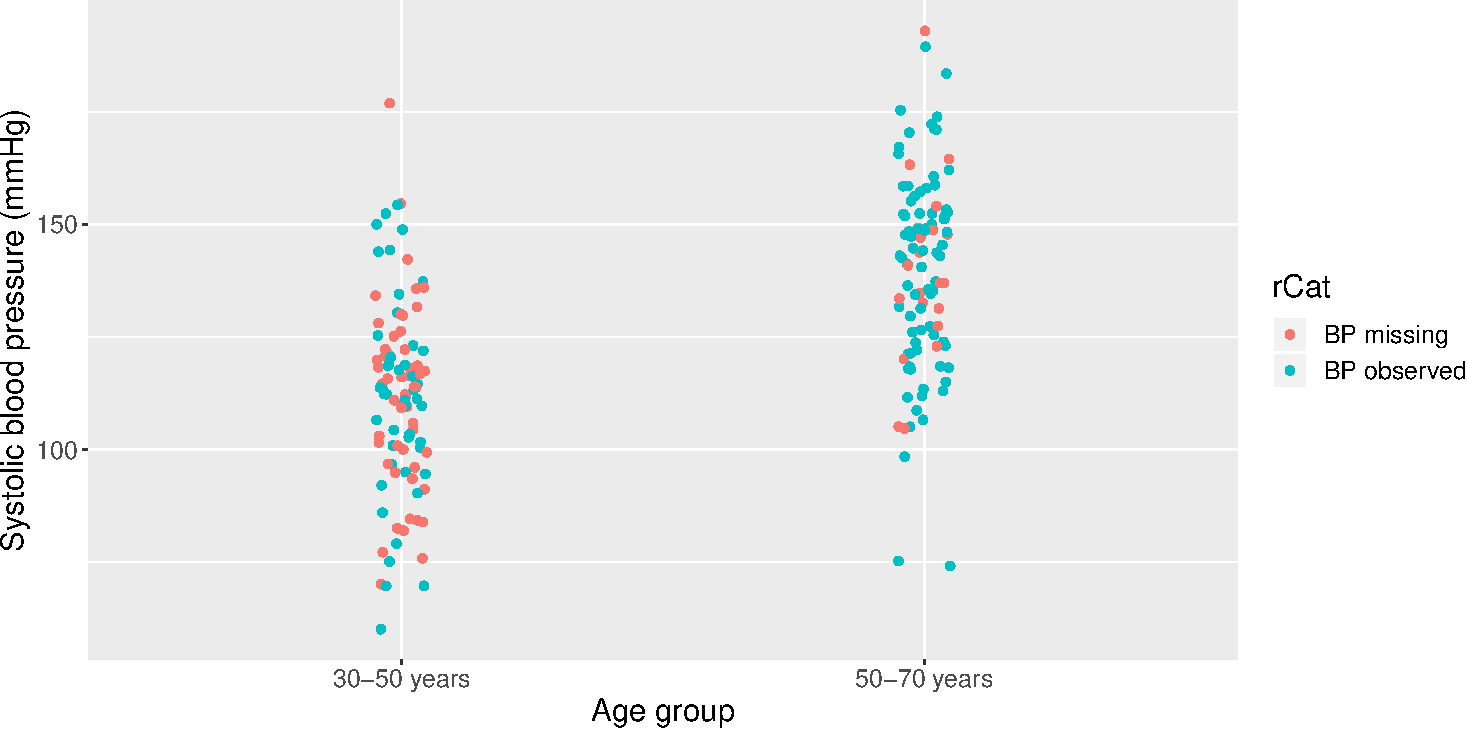
\includegraphics{Lecture1_files/figure-beamer/unnamed-chunk-5-1.pdf}

From this MAR appears plausible - within age categories, the
distributions of observed and missing BP look similar.

\end{frame}

\begin{frame}{Blood pressure MAR given age}
\protect\hypertarget{blood-pressure-mar-given-age-1}{}

But in reality all we get to see is:

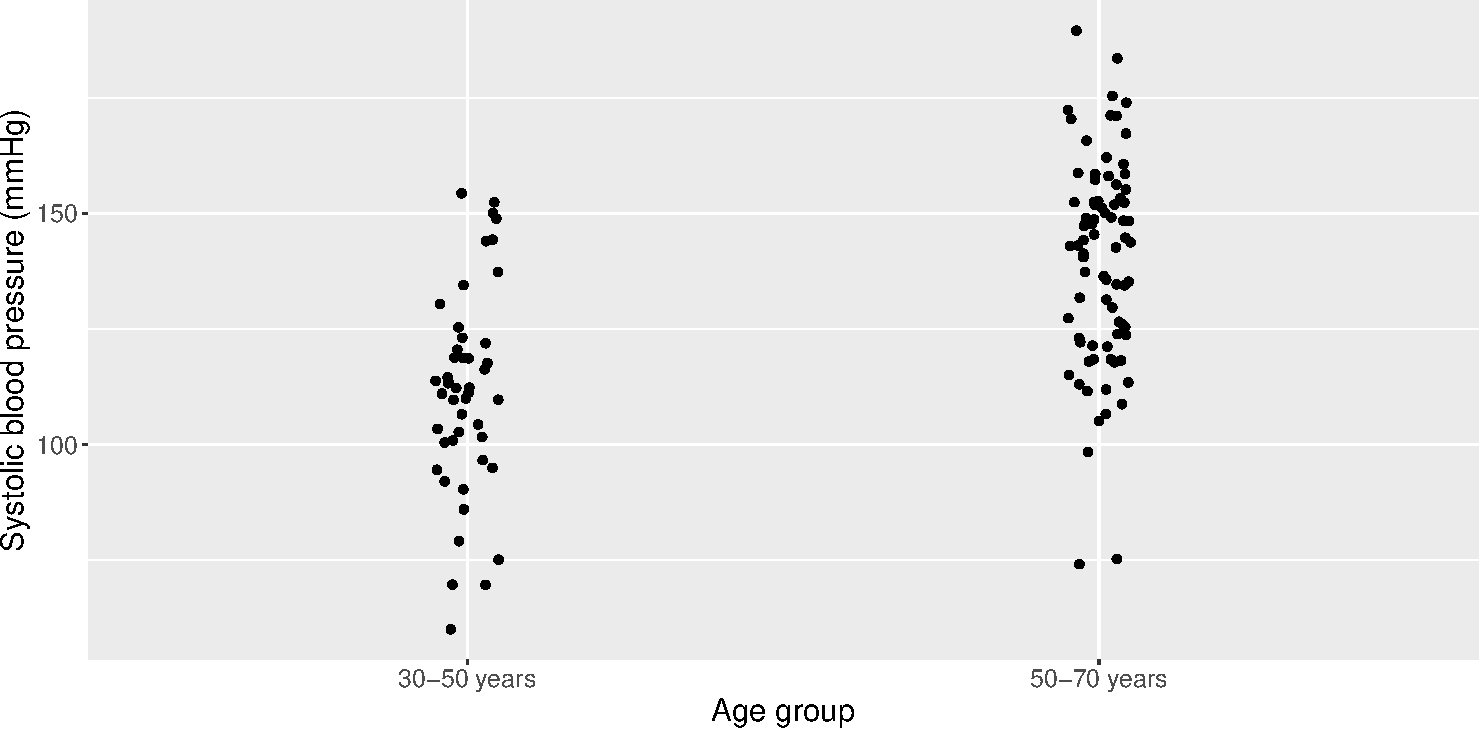
\includegraphics{Lecture1_files/figure-beamer/unnamed-chunk-6-1.pdf}

\end{frame}

\begin{frame}[fragile]{Analysis assuming MAR}
\protect\hypertarget{analysis-assuming-mar}{}

\begin{itemize}
\tightlist
\item
  If we are willing to assume data are MAR, we can construct unbiased
  estimates using a variety of statistical methods.
\item
  e.g.~estimate overall mean BP by a weighted average of observed BP
  means, weighting according to overall proportions of age categories:
\end{itemize}

\[  \frac{100 \times 111.4 + 100 \times 139.6}{200} = 125.5  \]

\begin{itemize}
\tightlist
\item
  Note this is not the same as crude average observed BP.
\end{itemize}

\small

\begin{Shaded}
\begin{Highlighting}[]
\KeywordTok{mean}\NormalTok{(bpObs}\OperatorTok{$}\NormalTok{bp, }\DataTypeTok{na.rm=}\OtherTok{TRUE}\NormalTok{)}
\end{Highlighting}
\end{Shaded}

\begin{verbatim}
## [1] 129.1174
\end{verbatim}

\normalsize

\end{frame}

\begin{frame}{A different representation of MAR}
\protect\hypertarget{a-different-representation-of-mar}{}

\begin{itemize}
\tightlist
\item
  We have defined MCAR and MAR in terms of how \(P(R=1|Y_{2},Y_{1})\)
  depends on age (\(Y_{1}\)) and BP (\(Y_{2}\)).
\item
  From the plot, we see that MAR can also be viewed in terms of the
  conditional distribution of BP (\(Y_{2}\)) given age (\(Y_{1}\)).
\item
  MAR implies that
\end{itemize}

\[  f(Y_{2}|Y_{1},R=0)=f(Y_{2}|Y_{1},R=1)=f(Y_{2}|Y_{1})\]

\begin{itemize}
\tightlist
\item
  That is, the distribution of BP (\(Y_{2}\)), given age (\(Y_{1}\)), is
  the same whether or not BP (\(Y_{2}\)) is observed.
\item
  This key consequence of MAR is directly exploited by \textbf{multiple
  imputation}.
\end{itemize}

\end{frame}

\begin{frame}{Missing not at random}
\protect\hypertarget{missing-not-at-random}{}

\begin{itemize}
\tightlist
\item
  If data are neither MCAR nor MAR, they are missing not at random
  (MNAR).
\item
  This means the chance of seeing \(Y_{2}\) depends on \(Y_{2}\), even
  after conditioning on \(Y_{1}\).
\item
  Equivalently, \(f(Y_{2}|Y_{1},R=0) \neq f(Y_{2}|Y_{1},R=1)\).
\item
  MNAR is much more difficult to handle. Essentially the data cannot
  tell us how the missing values differ to the observed values (given
  \(Y_{1}\)).
\item
  We are thus led to conducting sensitivity analyses.
\end{itemize}

\end{frame}

\begin{frame}{An MNAR analysis of mean blood pressure}
\protect\hypertarget{an-mnar-analysis-of-mean-blood-pressure}{}

\begin{itemize}
\tightlist
\item
  Suppose that, within age categories, the missing BPs are 10mmHg higher
  than the observed BPs.
\item
  \textcolor{red}{Given} this assumption, we can estimate mean BP by
  assuming the mean of the missing BPs are 10mmHg higher than predicted
  by MAR:
\end{itemize}

\[ \frac{47 \times 111.4 + 53 \times 121.4 + 79 \times 139.6 + 21 \times 149.6}{200} = 129.2\]

\begin{itemize}
\tightlist
\item
  Note that we must specify how we think the missing BPs differ to the
  observed values, based on our contextual knowledge.
\item
  The data \textbf{cannot} tell us how large this difference is!
\end{itemize}

\end{frame}

\begin{frame}{Summary}
\protect\hypertarget{summary}{}

\begin{itemize}
\tightlist
\item
  Missing data introduce ambiguity into the analysis, beyond the
  familiar sampling imprecision.
\item
  Extra assumptions about the missingness mechanism are needed to ensure
  valid estimates and inferences.
\item
  These assumptions can rarely be verified from the data at hand.
\item
  It is sensible to consider carefully possible missingness mechanisms,
  and formulate appropriate analyses.
\item
  Because we cannot be sure about the type of missingness mechanism at
  work, sensitivity analyses are important.
\end{itemize}

\end{frame}

\begin{frame}{Summary continued}
\protect\hypertarget{summary-continued}{}

\begin{itemize}
\tightlist
\item
  Missingness mechanisms fall into three broad classes: MCAR, MAR and
  MNAR.
\item
  Under MCAR, we obtain valid estimates and inferences by analysing the
  subset of subjects with no missing values.
\item
  Under MAR, we must allow for variables (somehow) which predict
  missingness.
\item
  MAR analyses can be done in a number of ways.
\item
  Multiple imputation is one such approach, which we will explore in
  this course.
\end{itemize}

\end{frame}

\begin{frame}[allowframebreaks]{References}
\protect\hypertarget{references}{}

\hypertarget{refs}{}
\leavevmode\hypertarget{ref-NRC2010}{}%
Council, National Research. 2010. \emph{The Prevention and Treatment of
Missing Data in Clinical Trials}. Washington, DC: National Academies
Press.

\leavevmode\hypertarget{ref-karahalios2012review}{}%
Karahalios, Amalia, Laura Baglietto, John B Carlin, Dallas R English,
and Julie A Simpson. 2012. ``A Review of the Reporting and Handling of
Missing Data in Cohort Studies with Repeated Assessment of Exposure
Measures.'' \emph{BMC Medical Research Methodology} 12 (1). BioMed
Central: 96.

\leavevmode\hypertarget{ref-Little2012}{}%
Little, Roderick J., Ralph D'Agostino, Michael L. Cohen, Kay Dickersin,
Scott S. Emerson, John T. Farrar, Constantine Frangakis, et al. 2012.
``The Prevention and Treatment of Missing Data in Clinical Trials.''
\emph{New England Journal of Medicine} 367 (14): 1355--60.
\url{https://doi.org/10.1056/NEJMsr1203730}.

\leavevmode\hypertarget{ref-Marston2010}{}%
Marston, L., J. R. Carpenter, K. R. Walters, R. W. Morris, I. Nazareth,
and I. Petersen. 2010. ``Issues in Multiple Imputation of Missing Data
for Large General Practice Clinical Databases.''
\emph{Pharmacoepidemiology and Drug Safety} 19: 618--26.

\leavevmode\hypertarget{ref-Rubin:1976}{}%
Rubin, D B. 1976. ``Inference and missing data.'' \emph{Biometrika} 63:
581--92.

\end{frame}

\end{document}
